\documentclass[9pt]{beamer}\usepackage[]{graphicx}\usepackage[]{color}
%% maxwidth is the original width if it is less than linewidth
%% otherwise use linewidth (to make sure the graphics do not exceed the margin)
\makeatletter
\def\maxwidth{ %
  \ifdim\Gin@nat@width>\linewidth
    \linewidth
  \else
    \Gin@nat@width
  \fi
}
\makeatother

\definecolor{fgcolor}{rgb}{0.345, 0.345, 0.345}
\newcommand{\hlnum}[1]{\textcolor[rgb]{0.686,0.059,0.569}{#1}}%
\newcommand{\hlstr}[1]{\textcolor[rgb]{0.192,0.494,0.8}{#1}}%
\newcommand{\hlcom}[1]{\textcolor[rgb]{0.678,0.584,0.686}{\textit{#1}}}%
\newcommand{\hlopt}[1]{\textcolor[rgb]{0,0,0}{#1}}%
\newcommand{\hlstd}[1]{\textcolor[rgb]{0.345,0.345,0.345}{#1}}%
\newcommand{\hlkwa}[1]{\textcolor[rgb]{0.161,0.373,0.58}{\textbf{#1}}}%
\newcommand{\hlkwb}[1]{\textcolor[rgb]{0.69,0.353,0.396}{#1}}%
\newcommand{\hlkwc}[1]{\textcolor[rgb]{0.333,0.667,0.333}{#1}}%
\newcommand{\hlkwd}[1]{\textcolor[rgb]{0.737,0.353,0.396}{\textbf{#1}}}%
\let\hlipl\hlkwb

\usepackage{framed}
\makeatletter
\newenvironment{kframe}{%
 \def\at@end@of@kframe{}%
 \ifinner\ifhmode%
  \def\at@end@of@kframe{\end{minipage}}%
  \begin{minipage}{\columnwidth}%
 \fi\fi%
 \def\FrameCommand##1{\hskip\@totalleftmargin \hskip-\fboxsep
 \colorbox{shadecolor}{##1}\hskip-\fboxsep
     % There is no \\@totalrightmargin, so:
     \hskip-\linewidth \hskip-\@totalleftmargin \hskip\columnwidth}%
 \MakeFramed {\advance\hsize-\width
   \@totalleftmargin\z@ \linewidth\hsize
   \@setminipage}}%
 {\par\unskip\endMakeFramed%
 \at@end@of@kframe}
\makeatother

\definecolor{shadecolor}{rgb}{.97, .97, .97}
\definecolor{messagecolor}{rgb}{0, 0, 0}
\definecolor{warningcolor}{rgb}{1, 0, 1}
\definecolor{errorcolor}{rgb}{1, 0, 0}
\newenvironment{knitrout}{}{} % an empty environment to be redefined in TeX

\usepackage{alltt}

\usepackage{framed}
\usepackage{alltt}
\usepackage{amsmath}
\usepackage{mathtools}
\usepackage{graphicx, color}
\usepackage{natbib}
\usepackage{verbatim}
\usepackage{hyperref}
\usepackage{mathptmx}
\usepackage{beamerthemesplit}
\usepackage{lipsum}

\graphicspath{{../report/figs/} }

\setbeamersize{text margin left=5pt,text margin right=5pt}
\parskip 3mm

\definecolor{firebrick}{RGB}{178,34,34}
\useinnertheme{circles,rounded}
\usecolortheme[named=firebrick]{structure}
\useoutertheme{smoothtree}
\setbeamertemplate{footline}[frame number]

\title{  Priorcovmatrix  }
\author{Ignacio Alvarez-Castro}
\institute[IESTA]{ Center of Statistical Research (IESTA) \\ Universidad de la Rep\'ublica, Uruguay.}
\date{LatinR2018 \\ 3rd - 5th September 2018. Universidad de Palermo, Argentina.
}



\IfFileExists{upquote.sty}{\usepackage{upquote}}{}
\begin{document}

 \frame{\titlepage}
 
\section{Introduction}

\frame{
\tableofcontents[hideallsubsections]
}

\AtBeginSection[] {
  \begin{frame}[plain]
    \tableofcontents[currentsection]
  \end{frame}
  \addtocounter{framenumber}{-1}
}


\frame{
		\frametitle{Introduction}
Covariance matrix estimation		
\begin{itemize} \itemsep2em
\item  Multivariate normal sampling models 
\item random-intercept, random-slope models 
\begin{eqnarray}
\nonumber y_{ij} &=& \beta_{0j} + \beta_{1j} x_{ij} + \beta_{2j}z_{ij} + \epsilon_{ij} \\
\nonumber  \begin{pmatrix} \beta_{0j} \\ \beta_{1j} \\ \beta_{2j} \end{pmatrix} &\sim&  N \left( \begin{pmatrix} \mu_{0} \\ \mu_{1} \\ \mu_{2} \end{pmatrix} , \Sigma \right) , \;\;\; \epsilon_{ij} \sim N(0, \sigma^2) 
%\nonumber \epsilon &\sim& N(0, \sigma^2) 
\end{eqnarray}
%\item \cite{ovaskainen2017make} includes covariance matrix priors for comunity data hierarchical models
\end{itemize}
}

\section{ Covariance matrix estimation }
\begin{frame}
\frametitle{Bird counts on Superior forests}
 The Natural Resources Research Institute (University of Minnesota Duluth) carry out monitoring program for study regional population trends of forest birds.
%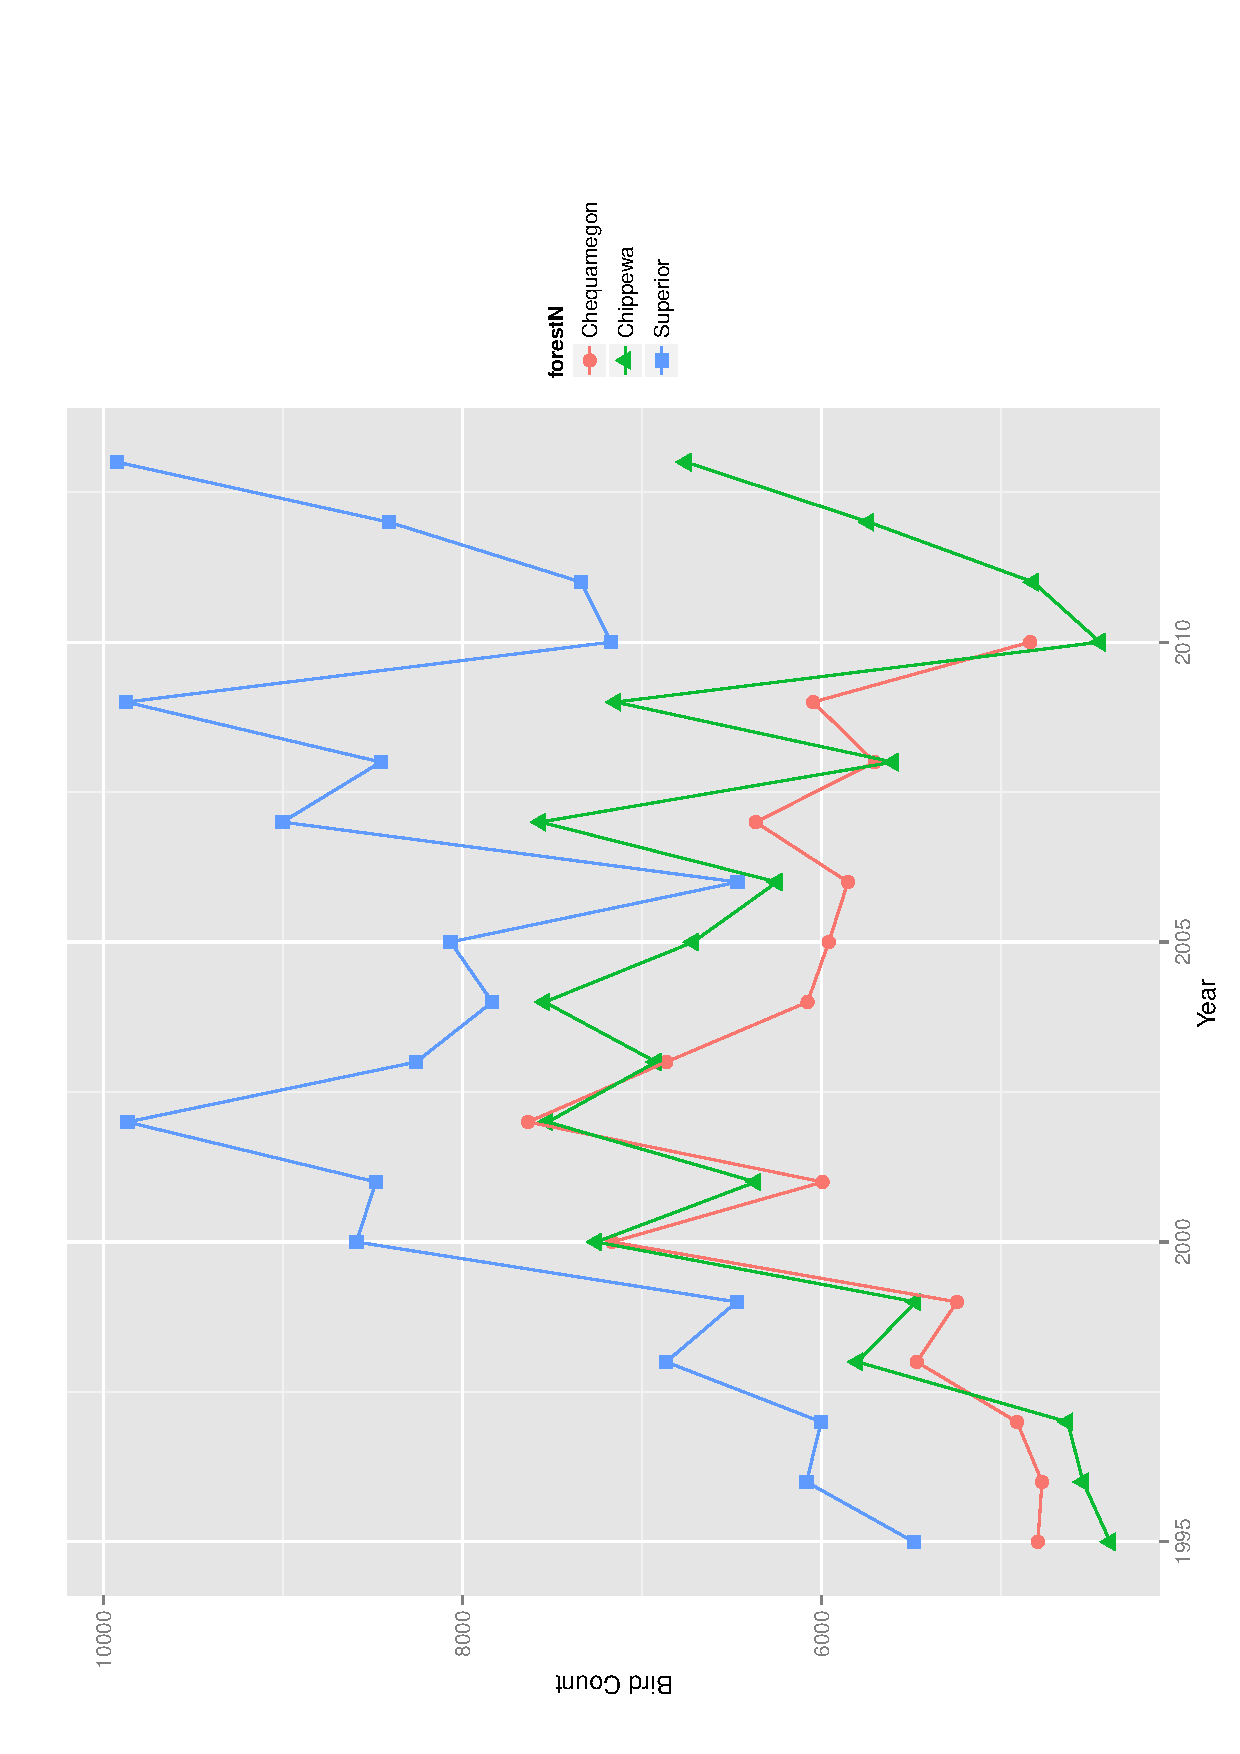
\includegraphics[width=\textwidth, height = 7cm ]{rawtrend}
\vspace{.5cm}

Want to study population trend over time
\[
E(y_{st})  = \beta_{0s} + \beta_{1s} t + \beta_{2t}t^2
\]

\begin{columns}
\begin{column}{4cm}
Point count for :
\begin{itemize}
  \item 19 years (1995 - 2013)
  \item 3 forest
  \item 73 bird species
\end{itemize}
\end{column}
\begin{column}{5cm}
Response $y_{st}$
\begin{itemize}
  \item Total count in logs
  \item Average count accros sites
  \item Total count
\end{itemize}

\end{column}
\end{columns}

\end{frame}


\begin{frame}
\frametitle{Quadratic trend model}

Hierarchical linear model with $IW$ prior.

\[\begin{array}{cl}
y_{st}  & \sim  N(\beta_{0s} + \beta_{1s} t + \beta_{2t}t^2, \sigma^2) \\
& \\
\begin{pmatrix} \beta_{0j} \\ \beta_{1j} \\ \beta_{2j} \end{pmatrix} & \sim  N \left( \begin{pmatrix} 0 \\ 0 \\ 0 \end{pmatrix} , \Sigma \right) \\
& \\
\Sigma & \sim  IW(d+1, I)
\end{array}
\]

Correlation among coefficient
\[ \rho = \Sigma_{23}/\sqrt{\Sigma_{22}\Sigma_{33}} \]

\end{frame}

\begin{frame}
\frametitle{Quadratic trend model}

Hierarchical linear model with $IW$ prior. Posterior $p(\rho | y)$

\begin{center}
\includegraphics[trim= 0cm 2cm 0cm 3cm, clip, scale=.7]{reg_3modIW}
\end{center}

\end{frame}

%============

\begin{frame}
\frametitle{ Multivariate normal model }

\cite{Alvarez2014} compare alternative priors for $\Sigma$ in this for multivariate normal data.
\[ Y_i \sim N_d(0, \Sigma) \]

Alternative $\Sigma$ priors
\begin{itemize}
\item Inverse Wishart: $IW(\nu, \Lambda)$:  $p(\Sigma) \propto  |\Sigma|^{-(\nu+ d +1)/2 } e^{-\frac{1}{2} tr( \Lambda \Sigma^{-1}) }$

\item Scaled Inverse Wishart
\item Hierarchical inverse Wishart
\item Separation strategy
\end{itemize}

Asses prior inpact on posterior inference:
\begin{itemize}
\item using simulations
\item with the bird count data set (not shown)
\end{itemize}
\end{frame}


\begin{frame}
\frametitle{Impact on posterior inference}
Inference for $\rho_{12}$
	\begin{columns}
	 \begin{column}{7cm}
		 \begin{figure}[hbtp]
		   \includegraphics[scale=.4]{fig_rho_d2}
		\end{figure}
	\end{column}
	\begin{column}{4cm}
	When standard deviation is small, $\sigma=0.01$ or $\sigma=0.1$ the IW prior heavily shrinks the posterior correlation towards 0 even if the true correlation is close to 1.
	\end{column}
	\end{columns}
\end{frame}

\section{R packages with STAN code (simulation) }

\begin{frame}[fragile]
\frametitle{Libraries with STAN code}

STAN: general purpuse sofware for Bayesian inference
\vspace{1cm} 

Set up package structure:
\begin{knitrout}
\definecolor{shadecolor}{rgb}{0.969, 0.969, 0.969}\color{fgcolor}\begin{kframe}
\begin{alltt}
\hlkwd{rstan_package_skeleton}\hlstd{(}\hlkwc{path} \hlstd{=} \hlstr{'PriorCovmatrix'}\hlstd{)}
\end{alltt}
\end{kframe}
\end{knitrout}

or
\begin{knitrout}
\definecolor{shadecolor}{rgb}{0.969, 0.969, 0.969}\color{fgcolor}\begin{kframe}
\begin{alltt}
\hlkwd{rstan_package_skeleton}\hlstd{(}\hlkwc{path} \hlstd{=} \hlstr{'PriorCovmatrix'}\hlstd{,}
                       \hlkwc{stan_files} \hlstd{=}\hlstr{'list of .stan files'}\hlstd{)}
\end{alltt}
\end{kframe}
\end{knitrout}
\end{frame}

\begin{frame}[fragile]
\frametitle{Libraries with STAN code}

STAN: general purpuse sofware for Bayesian inference
\vspace{1cm}

Install package for first time
\begin{knitrout}
\definecolor{shadecolor}{rgb}{0.969, 0.969, 0.969}\color{fgcolor}\begin{kframe}
\begin{alltt}
\hlstd{devtools}\hlopt{::}\hlkwd{install}\hlstd{(}\hlkwc{args} \hlstd{=} \hlstr{"--preclean"}\hlstd{)}
\end{alltt}
\end{kframe}
\end{knitrout}

or
\begin{knitrout}
\definecolor{shadecolor}{rgb}{0.969, 0.969, 0.969}\color{fgcolor}\begin{kframe}
\begin{alltt}
\hlstd{devtools}\hlopt{::}\hlkwd{install}\hlstd{()}
\end{alltt}
\end{kframe}
\end{knitrout}
\end{frame}


\begin{frame}[fragile]
\frametitle{Priorcovmatrix: starting point }

little funcionality so far
\begin{knitrout}
\definecolor{shadecolor}{rgb}{0.969, 0.969, 0.969}\color{fgcolor}\begin{kframe}
\begin{alltt}
\hlkwd{rIW}(n, d, R)

\hlkwd{rSS}(n, k prior_cor = \hlstr{'lkj'}, prior_sg =\hlstr{'ln'}, 
    eta = k+1, R = \hlkwd{diag}(k), sigma_mu=0, sigma_sc=1)

\hlkwd{covmat}(x, xnames = NULL, colvar = \hlstr{'dep'})
\end{alltt}
\end{kframe}
\end{knitrout}
\end{frame}

\section{ Visualize covariance matrix distribution }

\begin{frame}[fragile]
\frametitle{ Visualize a covariance matrix \textbf{distribution} }

\begin{itemize}
  \item not just one covariance matrix 
  \vspace{.1cm}
  \item reduce to bivariate pieces \citep{visualize}
  \vspace{.1cm}
  \item use scalar measures \citep{pena2003descriptive}
\end{itemize}

Parallel coordinate plot
\begin{itemize}
  \item all matrix entries in one plot
  \item use color to look for patterns
\end{itemize}

\end{frame}

\begin{frame}[fragile]
\frametitle{ Simulated example }

Simulate $n$ four-dimensional covariance matrices: $\Sigma \sim IW(d, R)$.  

\begin{tabular}{lcc}
 & parameter & values \\
 sample size & $n$ & 100 \\
 degrees of freedom & $d$ & 5, 15 \\
 correlation & $\rho$ & 0, 0.8
\end{tabular}
\vspace{1cm}

Location matrix is constructed as: 
\[ R =  \begin{pmatrix} 
1 & \rho & \rho & \rho \\ 
\rho & 1 & \rho & \rho \\ 
\rho & \rho & 1 &  \rho \\ 
\rho & \rho & \rho &1  \\ 
\end{pmatrix} \]

\end{frame}



\begin{frame}[fragile]
\frametitle{ Parallel coordinate plot: $\rho = 0 \;\; d=15$ }
\begin{knitrout}
\definecolor{shadecolor}{rgb}{0.969, 0.969, 0.969}\color{fgcolor}\begin{kframe}


{\ttfamily\noindent\itshape\color{messagecolor}{\#\# Joining, by = "{}grp.var"{}}}\end{kframe}\begin{figure}
\includegraphics[width=\maxwidth]{figure/unnamed-chunk-7-1} \caption[figura]{figura}\label{fig:unnamed-chunk-7}
\end{figure}


\end{knitrout}
\end{frame}

\begin{frame}[fragile]
\frametitle{ Parallel coordinate plot }
\begin{knitrout}
\definecolor{shadecolor}{rgb}{0.969, 0.969, 0.969}\color{fgcolor}
\includegraphics[width=\maxwidth]{figure/unnamed-chunk-8-1} 

\end{knitrout}

\end{frame}

\begin{frame}
\begin{center} Muchas Gracias ! \end{center}

\vspace{1.5cm}
\begin{itemize}
  \item @nachalca
  \item nachalca@iesta.edu.uy
  \item https://github.com/nachalca/PriorCovmatrix
\end{itemize}

\end{frame}

\begin{frame}
\frametitle{References}
  \bibliographystyle{../report/asa}      
\small{  \bibliography{../report/library} }
\end{frame}



\end{document}
